% This is the "preamble" of the document. This is where the format options get set.
% Pro-tip: things following the % mark will not be compiled by LaTeX. I'll be using them extensively to explain things as we go.
% Note: not to scare you off of LaTeX, but it's normal to have problems. And ya girl has been having some. I've included the copyright info at the bottom of the document from the guy who wrote this package, because his documentation doesn't entirely match how it's actually used. So this is a combination of his working preamble along with my added commentary or explanation. 
%% 

\documentclass[jou,12pt,floatsintext]{apa7}
% Document class input explanation ________________
% LaTeX files need to start with the document class, so it knows what it's using
% - This file is using the apa7 document class, as it has a lot of the formatting built in
% There are two sets of brackets in LaTeX, for each command (the things that start with the slash \ )
% - The squiggle brackets {} are mandatory for executing the command
% - The square brackets [] are options for that command. There can be more than one set of square brackets for some commands
% Options used in this document (general note - for each of these, if you want to use the other options, swap it out in that spot in the square brackets):
% - stu: this sets the `document mode' as the "student paper" version. Other options are jou (journal), man (manuscript, for journal submission), and doc (a plain document)
% --- The student setting includes things like 'duedate', 'course', and 'professor' on the title page. If these aren't wanted/needed, use the 'man' setting. It also defaults to including the tables and figures at the end of the document. This can be changed by including the 'floatsintext' option, as I have for you. If the instructor wants those at the end, remove that from the square brackets.
% --- The manuscript setting is roughly what you would use to submit to a journal, so uses 'date' instead of 'duedate', and doesn't include the 'course' or 'professor' info. As with 'stu', it defaults to putting the tables and figures at the end rather than in text. The same option will bump those images in text.
% --- Journal ('jou') outputs something similar to a common journal format - double columned text and figurs in place. This can be fun, especially if you are sumbiting this as a writing sample in applications.
% --- Document ('doc') outputs single columned, single spaced text with figures in place. Another option for producing a more polished looking document as a writing sample.
% - 12pt: sets the font size to 12pt. Other options are 10pt or 11pt
% - floatsintext: makes it so tables and figures will appear in text rather than at the end. Unfortunately, not having this option set breaks the whole document, and I haven't been able to figure out why. IT's GREAT WHEN THINGS WORK LIKE THEY'RE SUPPOSED TO.

\usepackage[american]{babel}
\usepackage{amsmath}
\usepackage{booktabs,caption}
\usepackage[flushleft]{threeparttable}

\usepackage{graphicx}
\graphicspath{ {./images/} }

\usepackage{csquotes} % One of the things you learn about LaTeX is at some level, it's like magic. The references weren't printing as they should without this line, and the guy who wrote the package included it, so here it is. Because LaTeX reasons.
\usepackage[style=apa,sortcites=true,sorting=nyt,backend=biber]{biblatex}
% biblatex: loads the package that will handle the bibliographic info. Other option is natbib, which allows for more customization
% - style=apa: sets the reference format to use apa (albeit the 6th edition)
\DeclareLanguageMapping{american}{american-apa} % Gotta make sure we're patriotic up in here. Seriously, though, there can be local variants to how citations are handled, this sets it to the American idiosyncrasies 
\addbibresource{bibliography.bib} % This is the companion file to the main one you're writing. It contains all of the bibliographic info for your references. It's a little bit of a pain to get used to, but once you do, it's the best. Especially if you recycle references between papers. You only have to get the pieces in the holes once.`
\setlength{\headheight}{14.49998pt}
\usepackage[T1]{fontenc} 
\usepackage{mathptmx} % This is the Times New Roman font, which was the norm back in my day. If you'd like to use a different font, the options are laid out here: https://www.overleaf.com/learn/latex/Font_typefaces
% Alternately, you can comment out or delete these two commands and just use the Overleaf default font. So many choices!
\usepackage{enumitem}

% Title page stuff _____________________
\title{The Interplay of Race/Ethnicity and Parental Education in Educational Attainment: A Cohort Analysis} % The big, long version of the title for the title page
\shorttitle{The Interplay of Race/Ethnicity \& Parental Education} % The short title for the header
\author{Christopher Byrd}
\date{March 16, 2026}
% \date{January 17, 2024} The student version doesn't use the \date command, for whatever reason
\authorsaffiliations{Whitworth University}

\abstract{Educational attainment is a key predictor of life outcomes. Despite this, access to opportunity within the American education system remains inequitable. This study examines how the intersectionality of race/ethnicity and parental education shape educational attainment among U.S. adults born between 1980 and 1984, using data from the National Longitudinal Survey of Youth 1997 (NLSY97). Prior research has highlighted racial disparities in school funding, disciplinary outcomes, and postsecondary access, as well as the effects of parental education on individual success. However, the interaction between the aforementioned variables remains under-explored in cohort-based analyses. This study applied multiple imputations and numerous logit models to investigate how educational attainment of residential parents, combined with race, influenced respondents' highest educational outcome completed by ages 33-37. Results indicate that while increased parental education is positively correlated with respondent educational attainment overall, the strength of this relationship varies significantly by race/ethnicity-parental interactions. Notably, Hispanic respondents demonstrated higher baseline odds of attainment but received smaller marginal benefits from increased parental education.}

\keywords{Educational Attainment, Structural Inequality, Race, Parental Education} % If you need to have keywords for your paper, delete the % at the start of this line
\renewcommand{\arraystretch}{0.9}
\begin{document}
\maketitle % This tells LaTeX to make the title page
\leftheader{The Interplay of Race/Ethnicity \& Parental Education}

\section{Introduction}

School serves as one of the most important institutions within an individual's life, affecting development and socialization \parencite[p.551-555]{conley_you_2019}. Throughout this experience, students of color are subjected to ethnic-racial discrimination. According to the UN Human Rights Office of the High Commissioner (OHCHR) (1965), ethnic-racial discrimination refers to negative behaviors experienced by individuals who identify as people of color. While often conceptualized as individual behavior, these experiences are rooted in systemic structures that disproportionally allocate social capital and resources. The effects of this discrimination are varied in reach and impact, from educational outcomes to adjustment within a school environment \parencite{bottiani_multilevel_2017, del_toro_when_2024, pearman_collective_2022}.

Additionally, parental educational attainment has been shown to impact their children's ability to succeed within an educational setting \parencite{assari_parental_2018,oakes_multiplying_1990,reed_educational_nodate}. This is made worse by the intersection of race \parencite{assari_parental_2018}. As such, it's important to consider how societal forces and structures affect differing educational outcomes, particularly with regard to parental educational achievement and ethnic-racial discrimination. Specifically, this analysis looks to answer the following question: among U.S. adults born from 1980 to 1984, how does the intersection of race/ethnicity and parental education affect the highest educational milestone completed by ages 33-37? This question is of particular interest as educational inequality is rampant in the United States and can affect all facets of life, from wealth to health \parencite{zajacova_relationship_2018, lurie_mechanisms_2021}. To answer this question, data from the National Longitudinal Survey of Youth 1997 (NLSY97), a comprehensive and nationally representative longitudinal survey, was analyzed utilizing multiple logit and binary regressions.

\section{The Literature}
\subsection{Availability of Resources}
The degree to which students and educators have access to resources significantly impacts student outcomes. \textcite{condron_disparities_2003} found a positive correlation between school spending and test scores, with schools serving predominantly minority and low-income populations consistently underfunded. Looking to the \textcite{national_center_for_education_statistics_concentration_2023}, over 30\% of Hispanic, Black, and Native students attend low-income schools, compared to only 7\% of White students. This stark disparity is often attributed to broader patterns of social stratification within U.S. society, with concrete examples within California's education system (\parencite{reed_educational_nodate, kozol_savage_1991}).

\textcite{oakes_multiplying_1990} argued that these inequities arise because inner-city schools lack the political influence needed to secure adequate funding. As a result, schools with a predominant minority student population often face severe resource deficits in science, thus limiting access to experienced teachers, adequate facilities, and technology necessary for academic success. It's notable that this article was prompted by a need for human capital—more workers in science and technology—and only partially driven by the intent to discover racial inequities.

\subsection{Belonging Within Schools}
\textcite{bottiani_multilevel_2017} completed a study that showed that gaps between White and Black students within out-of-school suspension (OSS) had a significant negative correlation on sense of belonging within a Black student's school. Alongside this was a positive correlation in adjustment problems with higher Black suspension rates. A higher low-SES population within a school also contributed to these findings, highlighting the importance of resources in student success. \textcite{king_examination_2011} found the opposite: school discipline had no effect on belonging and outcomes based upon race. This study is limited in scope, however, as it only examines whether there was discipline. There was no analysis of whether significant gaps existed based upon race.

\textcite{georgiades_emotional_2013} provided an interesting set of results in their study on belonging in school, emotional issues, and adjustment issues related to racial congruence and immigration generational status. For Asian and White students, an increase in congruence resulted in a negative correlation on behavioral problems, while the opposite was true for Black students (all groups being 3rd-generation immigrants). For emotional problems, we see a negative correlation for White and Black students when congruence increases, but a positive correlation for Asian students. The overall effects of congruence are very mixed. However, they are attenuated significantly by a sense of belonging, as this contributes directly to emotional and behavioral adjustment. That is to say, a sense of not belonging explains emotional and behavioral issues at a statistically significant level when a positive correlation is observed, rather than congruence.

Both studies contain parallels to critical race theory (CRT) and strain theory \parencite{bottiani_multilevel_2017, georgiades_emotional_2013, delgado_critical_2020}. Looking upon CRT, systemic inequalities, whether it be unequal representation in the student body, school punishment, or economic resources, increase racially divided outcomes in school performance, perpetuating negative stereotypes and increasing inequalities outside of schooling environments. Within strain theory, the pressures of belonging and increased punishment create strain upon students psyches and performance, resulting in the findings of \textcite{georgiades_emotional_2013}. Additionally, taking into account the social capital of parental education, lower parental attainment serves to increase the negative effects of both strain and critical race theory.

\subsection{School Achievement}
\subsubsection{Testing in Primary and Secondary Settings}
The Black-White score gap is a numerical manifestation of systemic inequities within education and society. \textcite{pearman_collective_2022} found that Black students are performing upwards of 0.5 standard deviations (SD) lower than their White peers, with this increasing modestly (0.1-0.2 SDs) with a SD of 1 or more with regard to county-level implicit and explicit bias. \textcite{del_toro_when_2024} found similarly that racist encounters with an educator, specifically in math, lead to lower test scores in both victimized students and students aware of the aggression. Students experiencing vicarious discrimination were subject to even lower scores than students directly affected, though the converse is true for class grades.

The score gap is also directly related to resources, where every additional \$1,000 in funding per student accounts for a subject-dependent increase of 6\%-10\% on state-administered standardized tests \parencite{condron_disparities_2003, reed_educational_nodate}. \textcite{reed_educational_nodate} found that clearance rates for the 10th grade exit test in California were appreciably lower in every race except Asians when compared to White students. Furthermore, over half of all Hispanic students were in low-performing schools, where there were 7\% fewer properly credentialed educators on staff.

\subsubsection{Post-Secondary Achievement and Family}
\textcite{reed_educational_nodate} found data supporting the concept that generational achievement affects outcomes for minority students. There is a correlation between the completion of secondary and post-secondary education by a mother and their four-year-old's likelihood to attend early childhood education (ECE) programs. According to \textcite{jones_benefits_2024},  there are significant benefits associated with attendance of ECE programs, amounting to higher wages and higher completion of education.

Moving back towards \textcite{reed_educational_nodate}, she finds that attenuating factors include general SES level, though SES is predicated often upon academic achievement. The general trend shows a vicious cycle of lower educational outcomes begetting lower educational outcomes. \textcite{assari_parental_2018} undertook a very similar study to the current one, finding that between Black and non-Hispanic White individuals, educational attainment was greater for White individuals, but educational mobility was higher for Black individuals. Furthermore, Assari included covariates for gender, finding these effects only occurred for female respondents.

\subsection{Theoretical Framework}
\subsubsection{Racial/Ethnic Generational Achievement \& Inequalities}

Through the late 1980s and early 1990s, Kimberlé Crenshaw (\citedate{crenshawMappingMarginsIntersectionality1991,crenshawDemarginalizingIntersectionRace1989}) developed a framework for analyzing the intersecting and additive effects of inequalities called Intersectionality. Intersectionality posits that simply examining inequalities experienced by an individual or group one-by-one is inadequate; rather, looking at how they work in tandem better explains the experiences and outcomes observed.

Additionally, a preeminent theory that attempts to explain segmentation in immigrant class outcomes and mobility is segmented assimilation theory, proposed by \textcite{portes_new_1993}. In their paper, Portes and Zhou examined second-generation immigrant households, arguing that not all immigrant groups follow the same upward trajectory of class mobility. Instead, assimilation pathways are shaped by numerous structural factors, such as race and community support structures. This often leads to outcomes that diverge in effects, from downward class mobility to assimilation of cultural ideas. These theories combined provide a valuable framework from which to observe the impact and effects of generational achievement. In particular, they help to explain how generational achievement may impact educational attainment differently depending on the social and institutional context in which families and individuals are embedded.

\subsection{Hypothesis}
From the available research and theory, the expected outcomes of the current study are as follows:

\begin{enumerate}[label=H\textsubscript{\arabic*}:]
  \item Higher levels of parental education and identifying as non-Black/non-Hispanic will independently lead to higher educational milestones completed by ages 33--37.
  \item The positive association between parental educational attainment and a respondent's own educational outcome will be significantly stronger for White individuals than for individuals of color.
  \item Specifically, it is expected that at higher levels of parental education, the attainment gap between non-Black/non-Hispanic respondents and Black or Hispanic respondents will persist or widen, suggesting that systemic racial discrimination attenuates the social capital typically provided by high parental education.
\end{enumerate}

\section{Methods}
\subsection{NLSY97 Survey Design, Sampling, and Participants}
As previously described, the sample used was the NLSY97 conducted by the US Bureau of Labor Statistics (BLS) (2024)\nocite{noauthor_nlsy97_nodate}. This is a nationally representative sample carried out every year pre-2011 and every two years thereafter, with selection finalized in 1997 and round 1 of questions carried out in 1998. This database was chosen due to the large sample size ($\textit{n} = 8,984$), robust and comprehensive question selection, representative nature (being weighted and stratified), and ease of access.

Individuals were chosen who were born between 1980 and 1984. At the time of first interviews, respondents' were ages 12 to 16. The sampling strategy, as described by the BLS, is as follows:
\begin{quote}
  “The NLSY97 cohort was selected in two phases... In the first phase, a list of housing units for the cross-sectional sample and the over-sample was derived from two independently selected, stratified multistage area probability samples. This ensured an accurate representation of different sections of the population defined by race, income, region, and other factors. In the second phase, sub-samples of the eligible persons identified in the first phase were selected for interview.”
\end{quote}
The longitudinal sample was used for all data analysis. Further information about the NLSY97 is available on the NLS website (2024).

\subsection{Measures}
\subsubsection{Respondent Education}
Within the NLSY97 (2024), the data was subset to specify participants in round 18 who responded with an answer to the following question: “[What is] the highest degree received as of the survey date?” This was on a scale of 0 to 7, with zero representing no high school completion and 7 representing a professional degree. All responses falling outside this range (non-interviews and invalid skips for respondents, ungraded for parents) were removed. This accounted for a removal of $\textit{n} = 2283$, with most being non-longitudinal respondents. Important to note is the difference in scales between parental and respondent education levels (see appendix A, table \ref{Tab:CODE} for the complete codebook).

Looking further into respondents HGC, there were two pairs of responses that posed a unique question with how to code: High School Diploma-GED and PhD-Professional degree (PD). Each pair provides similar results; a High School Diploma (HSD) and a GED both convey completion of grades K-12, whilst a PhD and PD are both terminal degrees. However, a HS Diploma and GED affect an individual's life course in differing ways, largely due to social stigma and age differences in attainment when compared to a diploma \parencite{maralaniGEDCollegeAge2011}. As such, HSD-GED were kept separated. On the contrary, the trajectory of PhD and PD are similar and were thus collapsed into a single response value. This resulted in a 0-6 scale. Additionally, any analysis that required removing the ordered factor structure from the variable resulted in a scale shifted by +1.

\subsubsection{Parental Education}

For parental education, residential parent (separated into mother and father - coded as "mom" and "dad") was chosen over biological, as the present study is concerned about the social power of education, not possible biological factors. As for coding, multiple approaches were considered. An analysis with parental education kept separate (additive effects) was tested but yielded results with high collinearity, suppression effects, and extremely high Variance Inflation Factor (VIF). For this reason, parental education was coded as the maximum between each residential pair. Where a residential parent was missing, education was coded as the education of the present parent. If both were missing, the response was coded as missing (\textit{NA}).

\subsubsection{Race and Ethnicity}
The NLSY97 offers a number of variables encoding race and/or ethnicity. For this analysis, the self-identified race/ethnicity key variable from round 1 was utilized. Round 4 contains seven dummy variables encoding race for the longitudinal sample; however, this increases the number of covariates sizeably and is interviewer-identified, whereas round 1 is self-identified. By forgoing the data from round 4, overfitting and implicit interviewer bias are avoided.

To test for effects, three dummy variables were coded (figure B) for race/ethnicity, with non-Black/non-Hispanic (NBNH) as the reference variable. This was done prior to imputation and was included in the predictor set.

\subsection{Imputations}

A unique aspect of the data that made analysis more complex was the number of answers missing from either one or both of the residential parent's educational attainment variable (round 1) (see appendix A). Figure \ref{Hist:Up} presents the missing data using an upset plot. An earlier analysis was completed with separated parent HGC values, which required imputation due to a casewise missingness of $\textit{n} = 2686$. After combining mother and father HGC to a single variable, missingness was reduced to $9\%$ or $\textit{n} = 79$.

Despite this reduction, imputations have been shown to produce better analyses than casewise deletion, especially when the data is MAR \parencite{afghari_contrasting_2019}. As such, Jamshidian and Jalal's (2010)\nocite{jamshidian_tests_2010} non-parametric Missing Completely at Random (MCAR) test was used to determine whether the pattern was random. Additionally, a number of sensitivity analyses were ran, ranging from regressing missing flags on observed values to comparing mean and SD values across parental pairs when accounting for missingness (See appendix for these analyses). These tests presented sufficient evidence for Missing At Random (MAR). Thus, all analyses proceeded under a MAR assumption.

Following this, data was imputed using the \textit{MICE} package, which utilizes Gibbs sampling \parencite{buuren_flexible_2021}. The imputation method chosen was predictive mean matching (PMM), as PMM provides plausible data that is robust given multiple data types \parencite{buuren_flexible_2021}. Twenty imputations ($\textit{m} = 20$) were conducted, with the model matrix including every covariate (see equation \ref{eq:Reg1.1}) and the dependent variable.

\subsection{Models}

All models featured the NLSY97 complex survey design, using sampling weights, strata, and primary sampling units (PSUs) via the \textit{svy} and \textit{svyVGAM} frameworks. Models were estimated and then pooled across imputations using Rubin's rules \parencite[Section 5.2]{buuren_flexible_2021}.

The primary model was a survey-weighted Proportional-odds Ordinal Logistic Regression (POLR). The following regression equation was used:

\begin{multline}
  \label{eq:Reg1.1}
  \text{logit}\left[P(Y_i \le k)\right] = \theta_k -
  \beta_1 \text{HGCParent}_i\\
  + \beta_2 \text{Black}_i
  + \beta_3 \text{Hispanic}_i
  + \beta_4 \text{Mixed}_i\\
  + \beta_5 (\text{HGCParent}_i \times \text{Black}_i)\\
  + \beta_6 (\text{HGCParent}_i \times \text{Hispanic}_i)\\
  + \beta_7 (\text{HGCParent}_i \times \\
  \text{Mixed}_i), \quad k=1,\dots,K-1.
\end{multline}

A secondary model featuring a quasibinomial logit was also tested for robustness checks. A passing value (1) was coded as achieving a degree of BA or higher. Quasibinomial was chosen over a standard binomial logit regression as the implementation of the standard binomial family in R fails to handle weights correctly. The following regression equation was used:
\begin{multline}
  \label{eq:Reg2}
  \text{logit}\left[P(\text{binaryHGC}_i=1)\right] =
  \alpha + \\
  \beta_1 \text{HGCParent}_i
  + \beta_2 \text{Black}_i
  + \beta_3 \text{Hispanic}_i\\
  + \beta_4 \text{Mixed}_i
  + \beta_5 (\text{HGCParent}_i \times \text{Black}_i)\\
  + \beta_6 (\text{HGCParent}_i \times \text{Hispanic}_i)\\
  + \beta_7 (\text{HGCParent}_i \times \text{Mixed}_i).
\end{multline}
Notably, stratum 117 presented only one PSU as a side effect of subsetting the data for model training. An analysis with the full dataset was conducted and presented similar results; as such, the training set was utilized and the mean for this stratum was set to the population mean.

\begin{table} \centering
  \begin{threeparttable}
    \caption{Number of Respondents and Highest Grade Completed by Race.}
    \label{Tab:Descriptive Res}
    \small
    \begin{tabular}{@{\extracolsep{5pt}} clccc}
      \toprule                                                      \\[-1.8ex]
      HGC  & Race                    & \textit{n} & Mean   & SD     \\
      \midrule                                                      \\[-1.8ex]
      None &                         &            & 127.75 & 84.06  \\
           & Black                   & 174        &        &        \\
           & Hispanic                & 161        &        &        \\
           & Mixed                   & 2          &        &        \\
           & NBNH\textsuperscript{1} & 174        &        &        \\
      GED  &                         &            & 215.25 & 154.99 \\
           & Black                   & 328        &        &        \\
           & Hispanic                & 179        &        &        \\
           & Mixed                   & 11         &        &        \\
           & NBNH                    & 343        &        &        \\
      HS   &                         &            & 672.5  & 495.84 \\
           & Black                   & 796        &        &        \\
           & Hispanic                & 655        &        &        \\
           & Mixed                   & 21         &        &        \\
           & NBNH                    & 1218       &        &        \\
      AA   &                         &            & 149.5  & 131.23 \\
           & Black                   & 144        &        &        \\
           & Hispanic                & 121        &        &        \\
           & Mixed                   & 8          &        &        \\
           & NBNH                    & 325        &        &        \\
      BA   &                         &            & 338    & 369.6  \\
           & Black                   & 256        &        &        \\
           & Hispanic                & 210        &        &        \\
           & Mixed                   & 16         &        &        \\
           & NBNH                    & 870        &        &        \\
      MA   &                         &            & 135    & 164.71 \\
           & Black                   & 99         &        &        \\
           & Hispanic                & 62         &        &        \\
           & Mixed                   & 4          &        &        \\
           & NBNH                    & 375        &        &        \\
      PhD* &                         &            & 37.25  & 45.31  \\
           & Black                   & 30         &        &        \\
           & Hispanic                & 14         &        &        \\
           & Mixed                   & 2          &        &        \\
           & NBNH                    & 103        &        &        \\
      \bottomrule                                                   \\[-1.8ex]
    \end{tabular}
    \normalsize
    \begin{tablenotes}
      \item \textit{Note.}
      \item *PhD and PD. \textsuperscript{1}NBNH = Non-Black Non-Hispanic.
    \end{tablenotes}
  \end{threeparttable}
\end{table}

\section{Results}

\subsection{Descriptive Statistics}

In total, 6701 individuals were included in the analysis from a possible 8,984. Of this, $50.9\%$ were White ($\textit{n}=3408$) with a mean education of $3.85$, $27.3\%$ were Black ($\textit{n}=1827$) with a mean education of $3.22$, $20.9\%$ were Hispanic ($\textit{n}=1402$) with a mean education of $3.20$, and $1.0\%$ were mixed ($\textit{n}=64$) with a mean education of $3.70$. The mode of education across the board was $3$ (HS Diploma). Table \ref{Tab:Descriptive Res} provides a breakdown, by race, of educational attainment of all respondents, alongside educational category averages.

\subsection{Inferential Statistics}

\begin{table} \centering
  \begin{threeparttable}
    \caption{Missing Data Patterns for Jamshidian and Jalal's MCAR Test.}
    \label{Tab:MCAR}
    \small
    \setlength{\tabcolsep}{4pt}
    \begin{tabular*}{\columnwidth}{@{\extracolsep{\fill}}ccccc@{}}
      \toprule \\[-1.8ex]
      & \multicolumn{3}{c}{Value is Missing?} &                                        \\
      \cline{2-4}                                                                      \\[-1.8ex]
      Pattern & HGC Res                               & HGC Mom & HGC Dad & \textit{n} \\
      \midrule                                                                         \\[-1.8ex]
      1       & Y                                     & N       & N       & 79         \\
      2       & Y                                     & Y       & Y       & 588        \\
      3       & Y                                     & Y       & N       & 296        \\
      4       & Y                                     & N       & Y       & 36         \\
      \bottomrule                                                                      \\[-1.8ex]
    \end{tabular*}
    \normalsize
    \begin{tablenotes}
      \item \textit{Note.}
      \item HGC = Highest Grade Completed.
    \end{tablenotes}
  \end{threeparttable}
\end{table}

When the data for parental education is separated, Jamshidian and Jalal's test detects the data is not MCAR, and significantly so (Table \ref{Tab:MCAR}). This provides partial evidence to suggest the data is MAR and has a pattern predicted by an observed variable(s). Secondly, mean and SD was relatively stable across categories (Table \ref{Tab:Sens}). Additionally, dad and mom missingness was significantly correlated with race. Dad missingness was also correlated with mom HGC; however, reversing the regression lead to no correlation. Besides the last regression, these results suggest a MAR mechanism. Additionally, assuming MNAR, when HGC was pooled for parents, it lead to a relatively small \textit{n} of cases where this MNAR mechanism could occur. Finally, sensitivity analyses on the POLR model revealed model stability across assumptions. Thus, the decision to continue using imputations was made.

\begin{table} \centering
  \begin{threeparttable}
    \caption{Sensitivity Analysis of Means and SD Against Father Missingness}
    \label{Tab:Sens}
    \small
    \setlength{\tabcolsep}{4pt}
    \begin{tabular*}{\columnwidth}{@{\extracolsep{5pt}} ccccccc}
      \toprule \\[-1.8ex]
      & \multicolumn{2}{c}{Dad HGC} & \multicolumn{2}{c}{Mom HGC} & \multicolumn{2}{c}{Race}\\
      \cline{2-3} \cline{4-5} \cline{6-7} \\[-1.8ex]
      Missing & Mean & SD & Mean & SD & Mean & SD \\
      \hline \\[-1.8ex]
      Missing & NA & NA & 12.1 & 2.7 & 2.2 & 1.3 \\
      Observed & 12.9 & 3.3 & 12.8 & 3.0 & 3.1 & 1.3 \\
      \cline{2-3} \\[-1.8ex]
      & \multicolumn{2}{c}{Mom Miss} & & & \\
      \cline{2-3} \\
      Missing  & 0.2 & 0.4 \\
      Observed & 0.1 & 0.2 \\
      \bottomrule \\[-1.8ex]
    \end{tabular*}
    \normalsize
    \begin{tablenotes}
      \item \textit{Note.}
      \item HGC = Highest Grade Completed.
    \end{tablenotes}
  \end{threeparttable}
\end{table}

It is important to note that any time an imputation is used, there is a chance bias and variability will be introduced which may not have existed in the dataset prior to the imputation (Buuren, 2018). However, the benefits of an imputation in the present study--capturing data, especially in categories with low response numbers--outweigh the drawbacks. The relative homogeneity in density between the imputed and observed values (Figues \ref{Dens:Imp}) supports the quality of the imputations, likely leading to less effect on the study outcome when compared to casewise deletion.

\begin{table*}[!t]
  \centering
  \begin{threeparttable}
    \caption{Survey-Weighted Proportional-Odds Logit Regression}
    \label{Tab:POLR}
    \setlength{\tabcolsep}{6pt}
    \begin{tabular*}{\textwidth}{@{\extracolsep{\fill}} lcccccc@{}}
      \toprule \\[-1.8ex]
      & & & & & \multicolumn{2}{c}{$95\%$ CI} \\
      \cline{6-7} \\[-1.8ex]
      & Log Odds & Odd Ratio & SE & Statistic\textsuperscript{1} & 2.5 \% & 97.5 \% \\
      \midrule \\[-1.8ex]
      HGCParent & $0.324$* & $1.382$ & $0.015$ & $21.719$ & $0.294$ & $0.353$ \\
      Black & $$-$0.274$ & $0.760$ & $0.533$ & $$-$0.514$ & $$-$1.335$ & $0.788$ \\
        Hispanic & $2.032$* & $7.633$ & $0.299$ & $6.792$ & $1.442$ & $2.623$ \\
        Mixed & $$-$0.850$ & $0.427$ & $1.421$ & $$-$0.598$ & $$-$3.661$ & $1.960$ \\
      HGCParent:Black & $$-$0.013$ & $0.987$ & $0.041$ & $$-$0.311$ & $$-$0.094$ & $0.069$ \\
        HGCParent:Hispanic & $$-$0.167$* & $0.846$ & $0.023$ & $$-$7.330$ & $$-$0.212$ & $$-$0.122$ \\
        HGCParent:Mixed & $0.021$ & $1.022$ & $0.089$ & $0.240$ & $$-$0.155$ & $0.198$ \\
      None\textbar GED & $1.356$* & - & $0.218$ & $6.223$ & $0.926$ & $1.786$ \\
      GED\textbar HS & $2.617$* & - & $0.209$ & $12.523$ & $2.205$ & $3.029$ \\
      HS\textbar AA & $4.635$* & - & $0.217$ & $21.316$ & $4.206$ & $5.064$ \\
      AA\textbar BA & $5.098$* & - & $0.220$ & $23.127$ & $4.663$ & $5.532$ \\
      BA\textbar MA & $6.657$* & - & $0.238$ & $27.986$ & $6.187$ & $7.126$ \\
      MA\textbar PhD & $8.361$* & - & $0.259$ & $32.287$ & $7.850$ & $8.872$ \\
      \bottomrule \\[-1.8ex]
    \end{tabular*}
    \begin{tablenotes}
      \item \textit{Note.}
      \item HGC = Highest Grade Completed.
      \item \textsuperscript{1}Wald Test.
      \item *$p<0.05$
    \end{tablenotes}
  \end{threeparttable}
\end{table*}

\subsubsection{POLR Model}

The results of the pooled POLR model (figure \ref{Tab:POLR}) reveals that three of the seven predictors are statistically significant at CI = 95\%, those being HGC of the residential parent ($p < 0.01$, $\alpha = 0.05$), the interaction effect of residential parent HGC and being Hispanic ($p < 0.01$, $\alpha = 0.05$), and being Hispanic ($p < 0.01$, $\alpha = 0.05$) (table 2). The effects of residential HGC is in line with the literature, with an odd ratio slightly above 1. This means the effect is rather mild, but still noticeable and prevalent.

Notably, being Hispanic is indicative of increased log odds. Furthermore, Hispanic residential parents see a decreased effect of parental education increasingly respondents educational attainment, with an odd ratio of 0.84 ($p < 0.01$, $\alpha = 0.05$).

Looking at the non-significant predictors in the POLR model, most have an intercept within $\pm 0.05$ of 0, suggesting that, even if these predictors (all race-parent variables with the exception of Hispanic) were significant, their effects compared to the reference group, non-White/non-Hispanic individuals, are minimal. Black and mixed race show predictor estimates that have slightly stronger negative correlation, but each have extremely high p-values and confidence intervals overlapping 0.

Unsurprisingly, the threshold estimates for education show that almost every jump between educational levels have non-overlapping cutpoints, with the exception of HS|AA and AA|BA. This is possibly due to the strong emphasis on college completion in the US. Additionally, this lends credance to keeping GED and HS separate.

\begin{table*}[!t]
  \centering
  \begin{threeparttable}
    \caption{Survey-Weighted Quasibinomial Logit Regression}
    \label{Tab:BiLogit}
    \setlength{\tabcolsep}{6pt}
    \begin{tabular*}{\textwidth}{@{\extracolsep{\fill}} lcccccc@{}}
      \toprule \\[-1.8ex]
      & & & & & \multicolumn{2}{c}{$95\%$ CI} \\
      \cline{6-7} \\[-1.8ex]
      & Log Odds & OR & SE & Statistic\textsuperscript{1} & 2.5 \% & 97.5 \% \\
      \midrule \\[-1.8ex]
      (Intercept) & $$-$5.697$* & $0.003$ & $0.336$ & $$-$16.962$ & $$-$6.363$ & $$-$5.031$ \\
      HGCParentEd & $0.365$* & $1.441$ & $0.022$ & $16.711$ & $0.322$ & $0.409$ \\
      Black & $0.443$ & $1.557$ & $0.716$ & $0.619$ & $$-$0.984$ & $1.870$ \\
        Hispanic & $1.661$* & $5.263$ & $0.538$ & $3.087$ & $0.593$ & $2.728$ \\
        Mixed & $2.817$ & $16.721$ & $1.904$ & $1.479$ & $$-$0.986$ & $6.620$ \\
      HGCParent:Black & $$-$0.059$ & $0.942$ & $0.052$ & $$-$1.134$ & $$-$0.164$ & $0.045$ \\
        HGCParent:Hispanic & $$-$0.141$* & $0.868$ & $0.040$ & $$-$3.556$ & $$-$0.220$ & $$-$0.062$ \\
        HGCParent:Mixed & $$-$0.217\dagger$ & $0.805$ & $0.120$ & $$-$1.804$ & $$-$0.457$ & $0.023$ \\
      \bottomrule \\[-1.8ex]
    \end{tabular*}
    \begin{tablenotes}
      \item \textit{Note.}
      \item HGC = Highest Grade Completed.
      \item \textsuperscript{1}Wald Test.
      \item *$p<0.05$
      \item $\dagger p<0.10$
    \end{tablenotes}
  \end{threeparttable}
\end{table*}

\subsection{Quasibinomial Logit Model}

The quasibinomial model (figure \ref{Tab:BiLogit}) presents slightly divergent results. Significance is similar across the board, with the exception of the interaction of parental education and Mixed race, with a slightly negative log odd and marginally lower p-value ($p < 0.10$, $\alpha = 0.05$). Additionally, the predictive power of being Hispanic was lower when compared with the POLR model.

\section{Discussion}

Overall, the data partially supports and refutes the test hypotheses. Thus, H\textsubscript{1} is partially refuted, while H\textsubscript{2} and H\textsubscript{3} received mixed support depending on racial/ethnic group. While it's true that higher grade completion from a residential parent positively affects educational attainment, when interacting with race, White individuals do not see significant benefits of HGC from their parent over individuals of other races and ethnicities--with the exception of Hispanic individuals, who experience reduced benefits from parental HGC. However, when not accounting for parental HGC, Hispanic individuals have increased log-odds of achieving higher education.

\subsection{Parental Education: A Universal Driver of Higher Education}

Consistent with the literature, higher residential parental HGC significantly predicts increased educational attainment ($OR=1.382, p<0.01, \alpha=0.95$) \parencite{reed_educational_nodate,jones_benefits_2024,assari_parental_2018}. While modest, this effect predicts that, with each additional grade completed by a parent, the odds that their child will progress to a higher educational milestone increases by $38\%$.

The literature on educational transmission suggests this effect should be stronger among White families \parencite{oakes_multiplying_1990, assari_parental_2018}, yet the POLR and quasibinomial models show no significant effect differences by race for the Black and Mixed race groups. This pattern itself is notable: it suggests that while parental education matters universally, it matters in similar ways across racial groups.

\subsection{Education and Identifying as Hispanic}

Using segmented assimilation theory \parencite{portes_new_1993}, it is possible that the results we see from Hispanic individuals come from a multitude of societal and familial structures. Previous research shows Hispanic educational attainment (AA or above) to be severely below that of many other racial groups in the US, particularly White \parencite{kim_race_2024}. We are beginning to see increases in the rates at which Hispanic individuals attain higher education, and while these rates may not be high compared to the general population (48.1\% versus 29.5\%), segmented outcomes in the individuals studied can possibly explain the results. These segmentations could arise in multiple fashions. For example, this could be due to the citizenship status of individuals surveyed and whether this proportion is generalizable to the US population of Hispanic individuals. This may also align with findings on immigrant optimism, where high educational aspirations persist notwithstanding socioeconomic disadvantages \parencite{kaoOptimismAchievementEducational2022}, potentially driving attainment independently of parental HGC.

Furthermore, \textcite{kaoOptimismAchievementEducational2022} found that the immigration status of Hispanic individuals is less important to educational achievement. This may be due in part from societal or cultural barriers which prevent the full relation of educational capital from parent to child in Hispanic families. The findings suggest that simply improving parental education levels may not equitably improve intergenerational mobility for all racial groups. Educational policy must then address these societal/cultural barriers and structures, should they be present.

\subsection{Interactions for Black and Mixed-Race Respondents}

Contrary to H\textsubscript{2} and H\textsubscript{3}, Black respondents show no significant interactions between parental education and educational attainment (OR = $0.987$, $p > 0.10$), and Mixed race respondents similarly show no significant effect in the POLR model. A possible explanation for these results lies in \textcite{bottiani_multilevel_2017}, who found that discipline gaps negatively correlated with school belonging, mediated by school-wide SES. It's possible that the barriers depicted here are so pervasive they prevent the upwards effects of parental education from appearing.

The extremely small sample of Mixed race respondents ($n=64$) makes interpretability difficult for this group, as noted in limitations. However, the pattern of non-significance across both Black and Mixed groups suggests that intersectionality operates selectively between the reference group and focus groups; it emerges strongly for Hispanic respondents but not for other groups. This mechanism warrants further research into the conditions under which intersectional processes are observable or significant in quantitative data.

\subsection{Limitations}
As previously noted, imputations can introduce error into analyses from inconsistent, variable data, possibly affecting results. Furthermore, measures drawn from imputed data rely upon proper model specification and a MAR or MCAR assumption. However, given the percent of missing and density graph, there is sufficient evidence to support the quality of the imputation. Additionally, an increased amount of runs serves to reduce variability in the observed effects of fitted models.

Furthermore, GED and HS are interpreted as discrete ordinal categories, with GED placed below HS. While societally they may be seen as different, practically, they hold similar functional distinction. On the other hand, a PhD and a professional degree were collapsed into a single level (level 7). See \textit{methods}.

Looking at the various models, a lack of additional covariates serves to prevent overfitting; however, it can also prevent the full picture from becoming evident. Given the relatively high VIF present in the current study, it's recommended that future papers utilize dimensionality reduction techniques or regularization with an increase in covariates.

Lastly, the sample size for individuals of mixed race is excessively small ($\textit{n}=64)$ after selecting valid cases and prior to casewise deletion or imputation of invalid/missing parent HGC answers. As such, large uncertainty and low prediction validity was expected. Future studies should aim to encapsulate a greater number of respondents within this demographic, as it is underexplored.

\subsection{Implications for Future Research}

Future research should expand upon the present study by including confounders which may create more generalizable results, such as increasing covariates. Additionally, a longitudinal study tailored specifically to researching the intersectionality of race and parental education may yield better results. Segmenting race and ethnicity further may allow a more nuanced view of racial-ethnic divides in attainment. Furthermore, future research may seek to define educational success along the lines of educational achievement and job status, as education is only one small part in a person's wellbeing. With regards to ethnic and racial groups, future studies should attempt to identify societal and cultural factors which moderate gains or decreases in attainment.

\section{Conclusions}

This study contributes to the educational inequality literature by presenting that not only do disparities exist, but how and for whom educational capital strengthens outcomes across generations. The results demonstrate that intersectionality operates selectively, with results and significance that vary by racial/ethnic group. Hispanic respondents present an intriguing outcome of high baseline attainment coupled with restrained parental education effects, possibly reflecting immigrant optimism and within-group heterogeneity. Black respondents show uniform constraint across all parental education levels, consistent with theories of pervasive structural racism. These patterns highlight that reducing educational inequality requires moving beyond individual- or family-level interventions to address the institutional structures that shape opportunity inequitably across racial and ethnic groups.

\printbibliography

\onecolumn
\appendix

\section{Codebook}

\begin{table}[h] \centering
  \begin{threeparttable}
    \caption{Codebook of Variables.}
    \label{Tab:CODE}
    \small
    \setlength{\tabcolsep}{4pt}
    \begin{tabular*}{\columnwidth}{@{\extracolsep{\fill}}crlcrl@{}}
      \toprule \\[-1.8ex]
      Var & \multicolumn{2}{c}{Key} & Var & \multicolumn{2}{c}{Key} \\
      \midrule \\[-1.8ex]
      HGC Mom \& Dad  & & &*Race \& Ethnicity & & \\
      & 0 & None &  & 1 & Black \\
      & 1 & 1st & & 2 & Hispanic \\
      & 2 & 2nd & & 3 & Mixed \\
      & 3 & 3rd & & 4 & NBNH \\
      & 4 & 4th & & & \\
      & 5 & 5th & & & \\
      & 6 & 6th & & & \\
      & 7 & 7th & & & \\
      & 8 & 8th & & & \\
      & 9 & 9th & & & \\
      & 10 & 10th & & & \\
      & 11 & 11th & & & \\
      & 12 & 12th & & & \\
      & 13 & 13th & & & \\
      & 14 & 14th & & & \\
      & 15 & 15th & & & \\
      & 16 & 16th & & & \\
      & 17 & 17th & & & \\
      & 18 & 18th & & & \\
      & 19 & 19th & & & \\
      & 20 & 20th & & & \\
      \bottomrule \\[-1.8ex]
    \end{tabular*}
    \normalsize
    \begin{tablenotes}
      \item HGC = Highest Grade Completed.
      \item NBNH = Non-Black Non-Hispanic.
      \item *These variables are raw NLSY97 data and are mutated prior to use in the paper.
    \end{tablenotes}
  \end{threeparttable}
\end{table}

\section{Expanded Demographics and Figures}

\begin{figure*}
  \caption{Highest Grade Completion of Respondant by Race.}
  \label{Hist:Resp}
  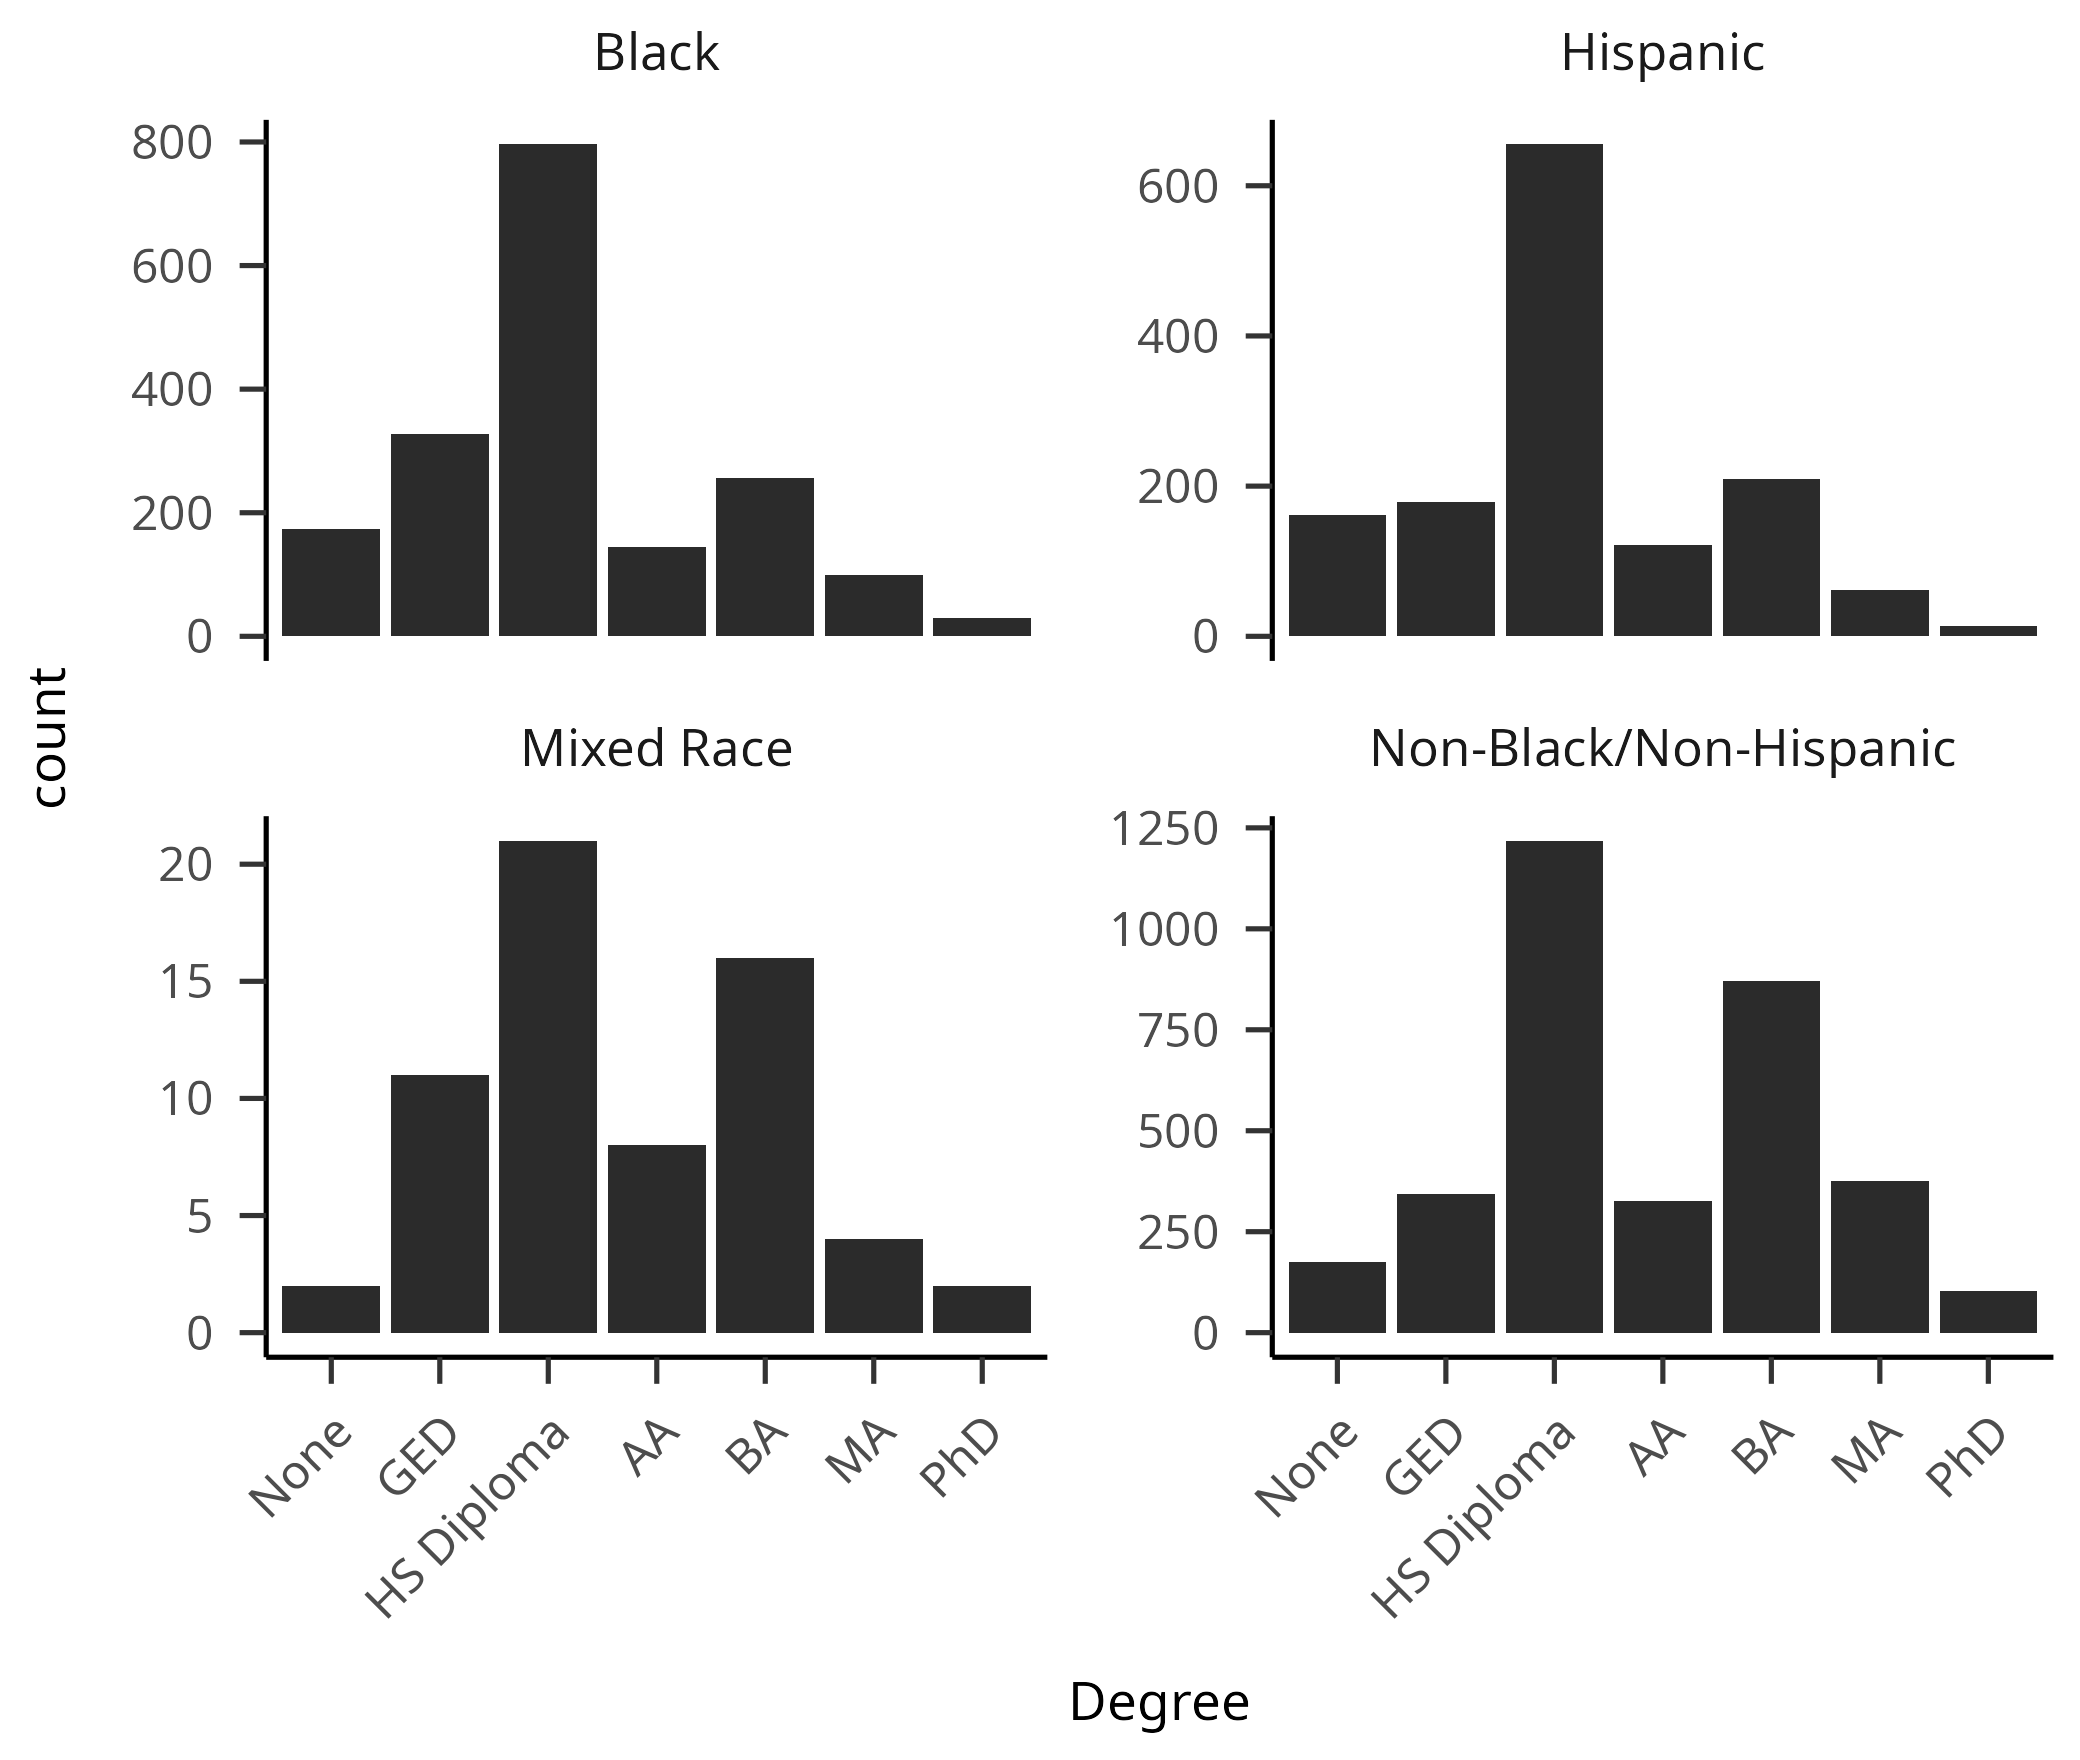
\includegraphics[width=\textwidth]{histogram}
\end{figure*}

\begin{figure*}
  \caption{Highest Grade Completion of Residential Mom by Race.}
  \label{Hist:Mom}
  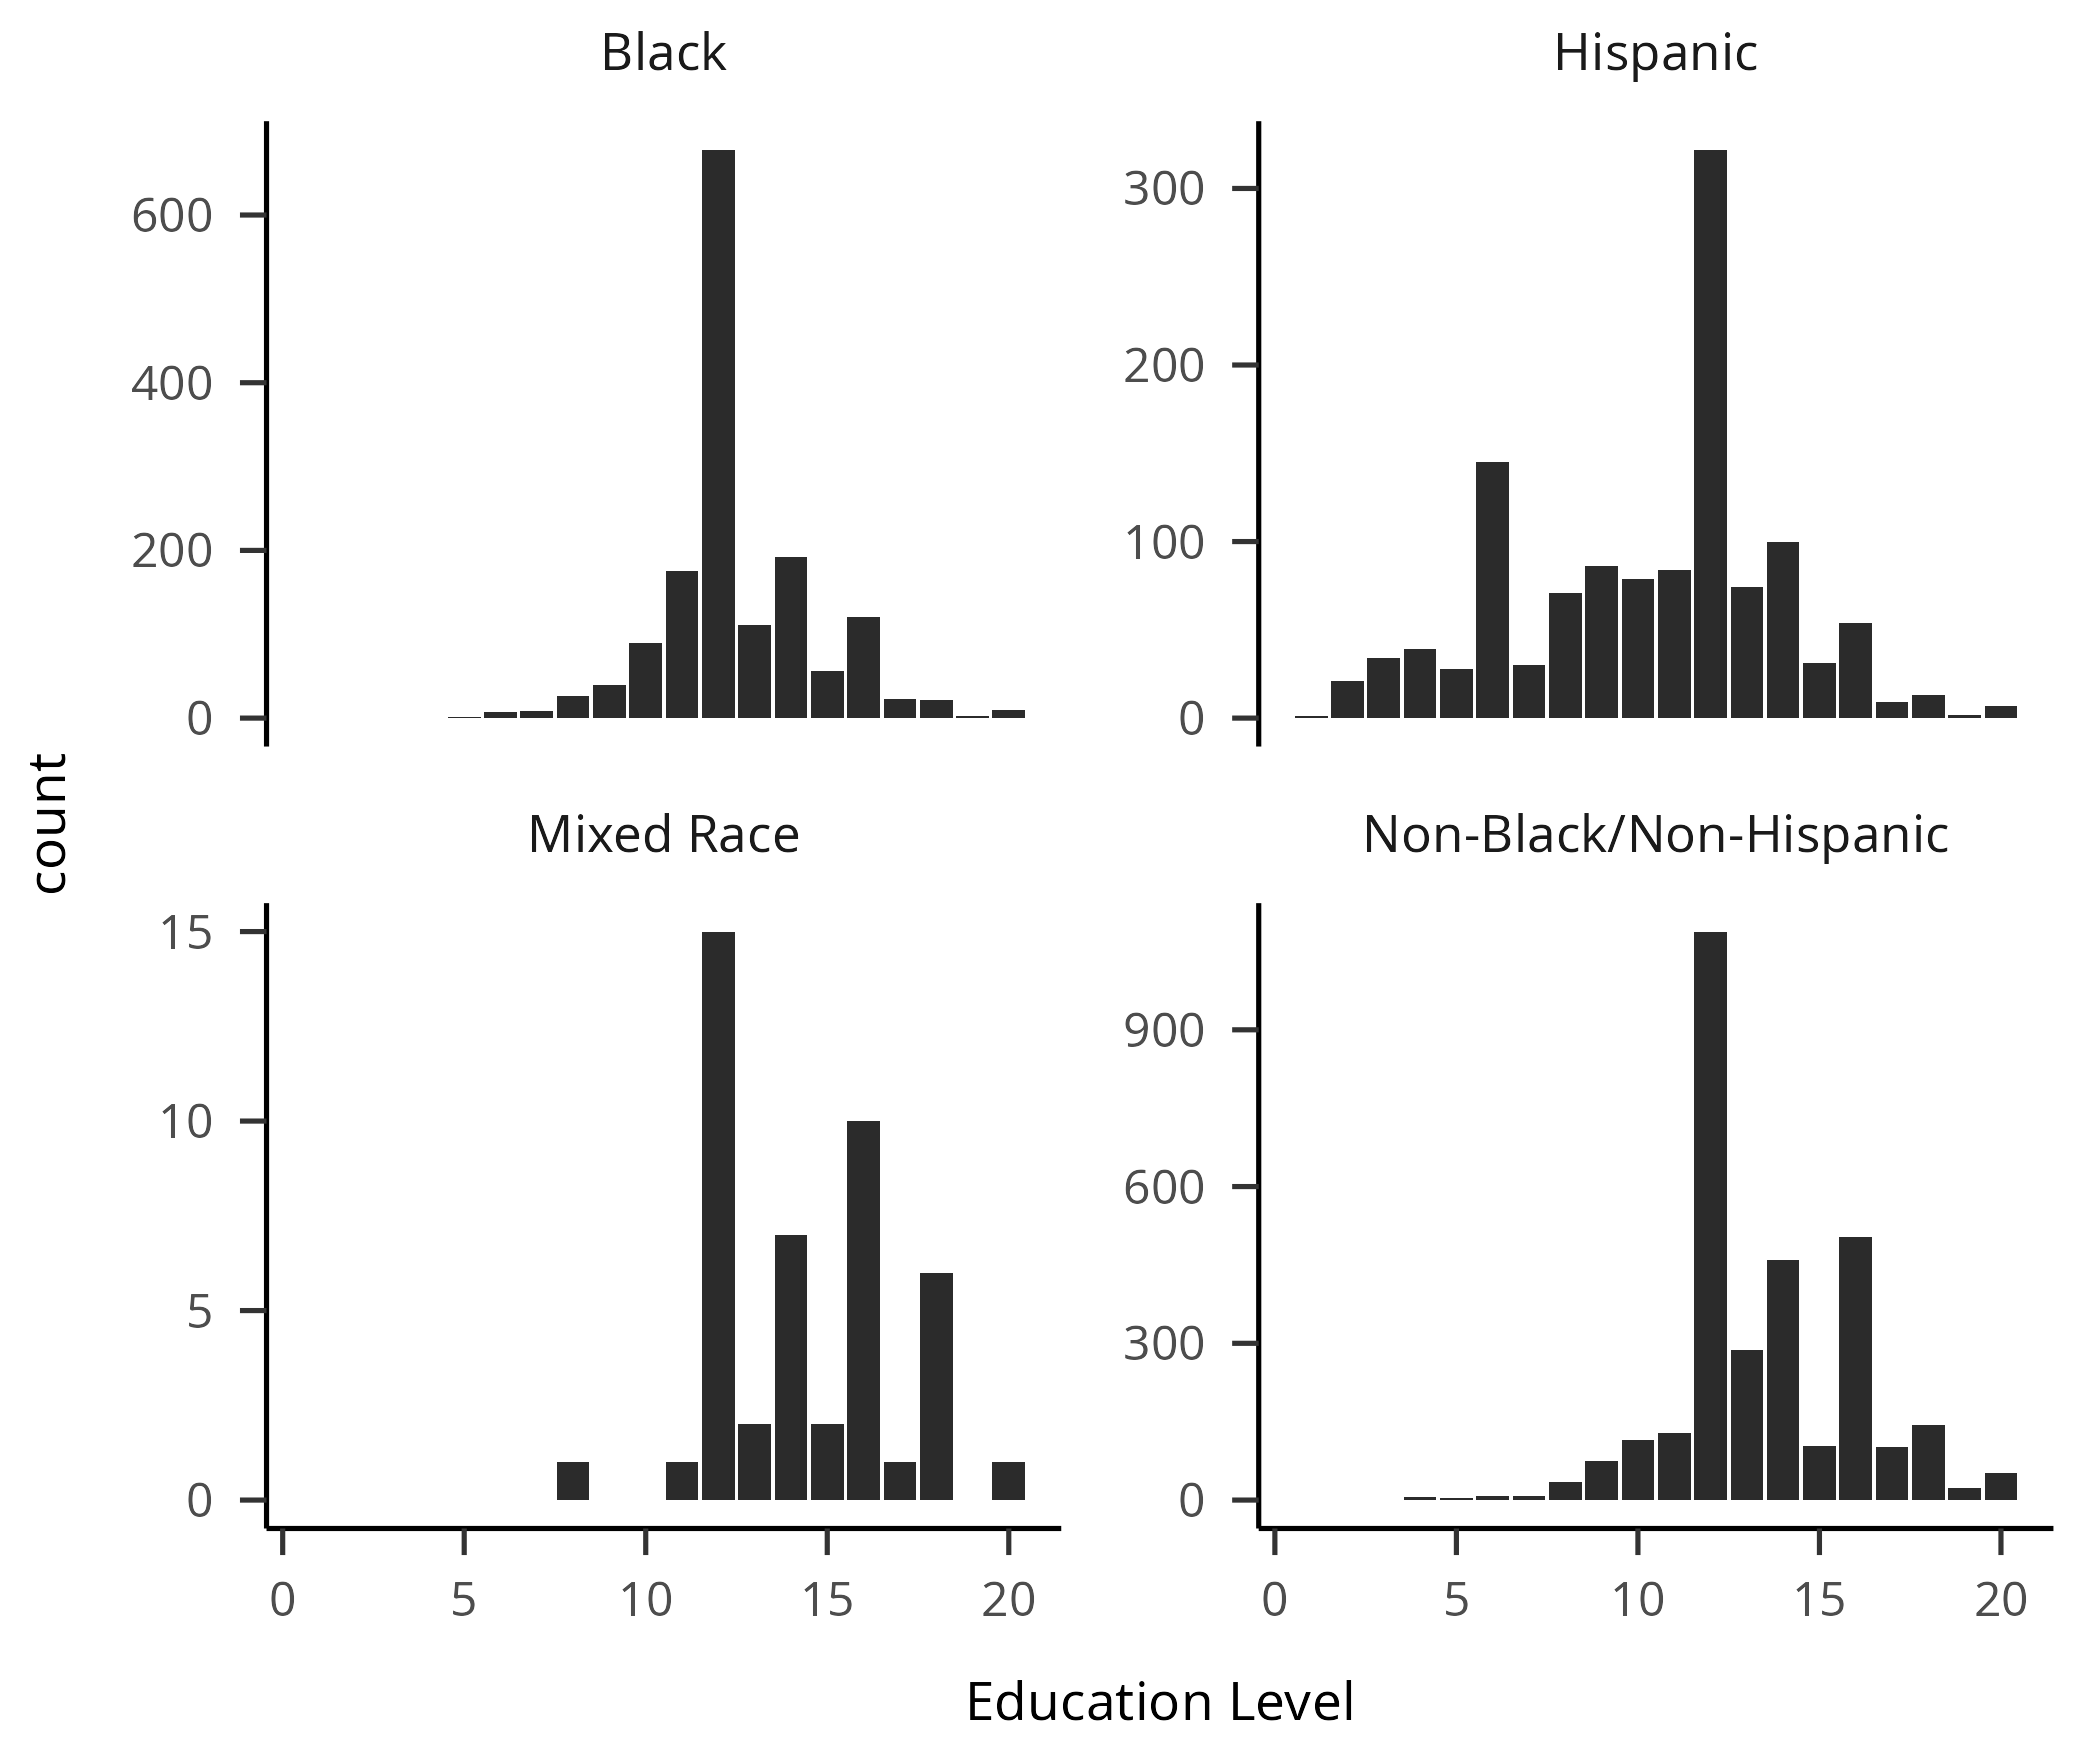
\includegraphics[width=\textwidth]{histogram2}
\end{figure*}

\begin{figure*}
  \caption{Highest Grade Completion of Residential Dad by Race.}
  \label{Hist:Dad}
  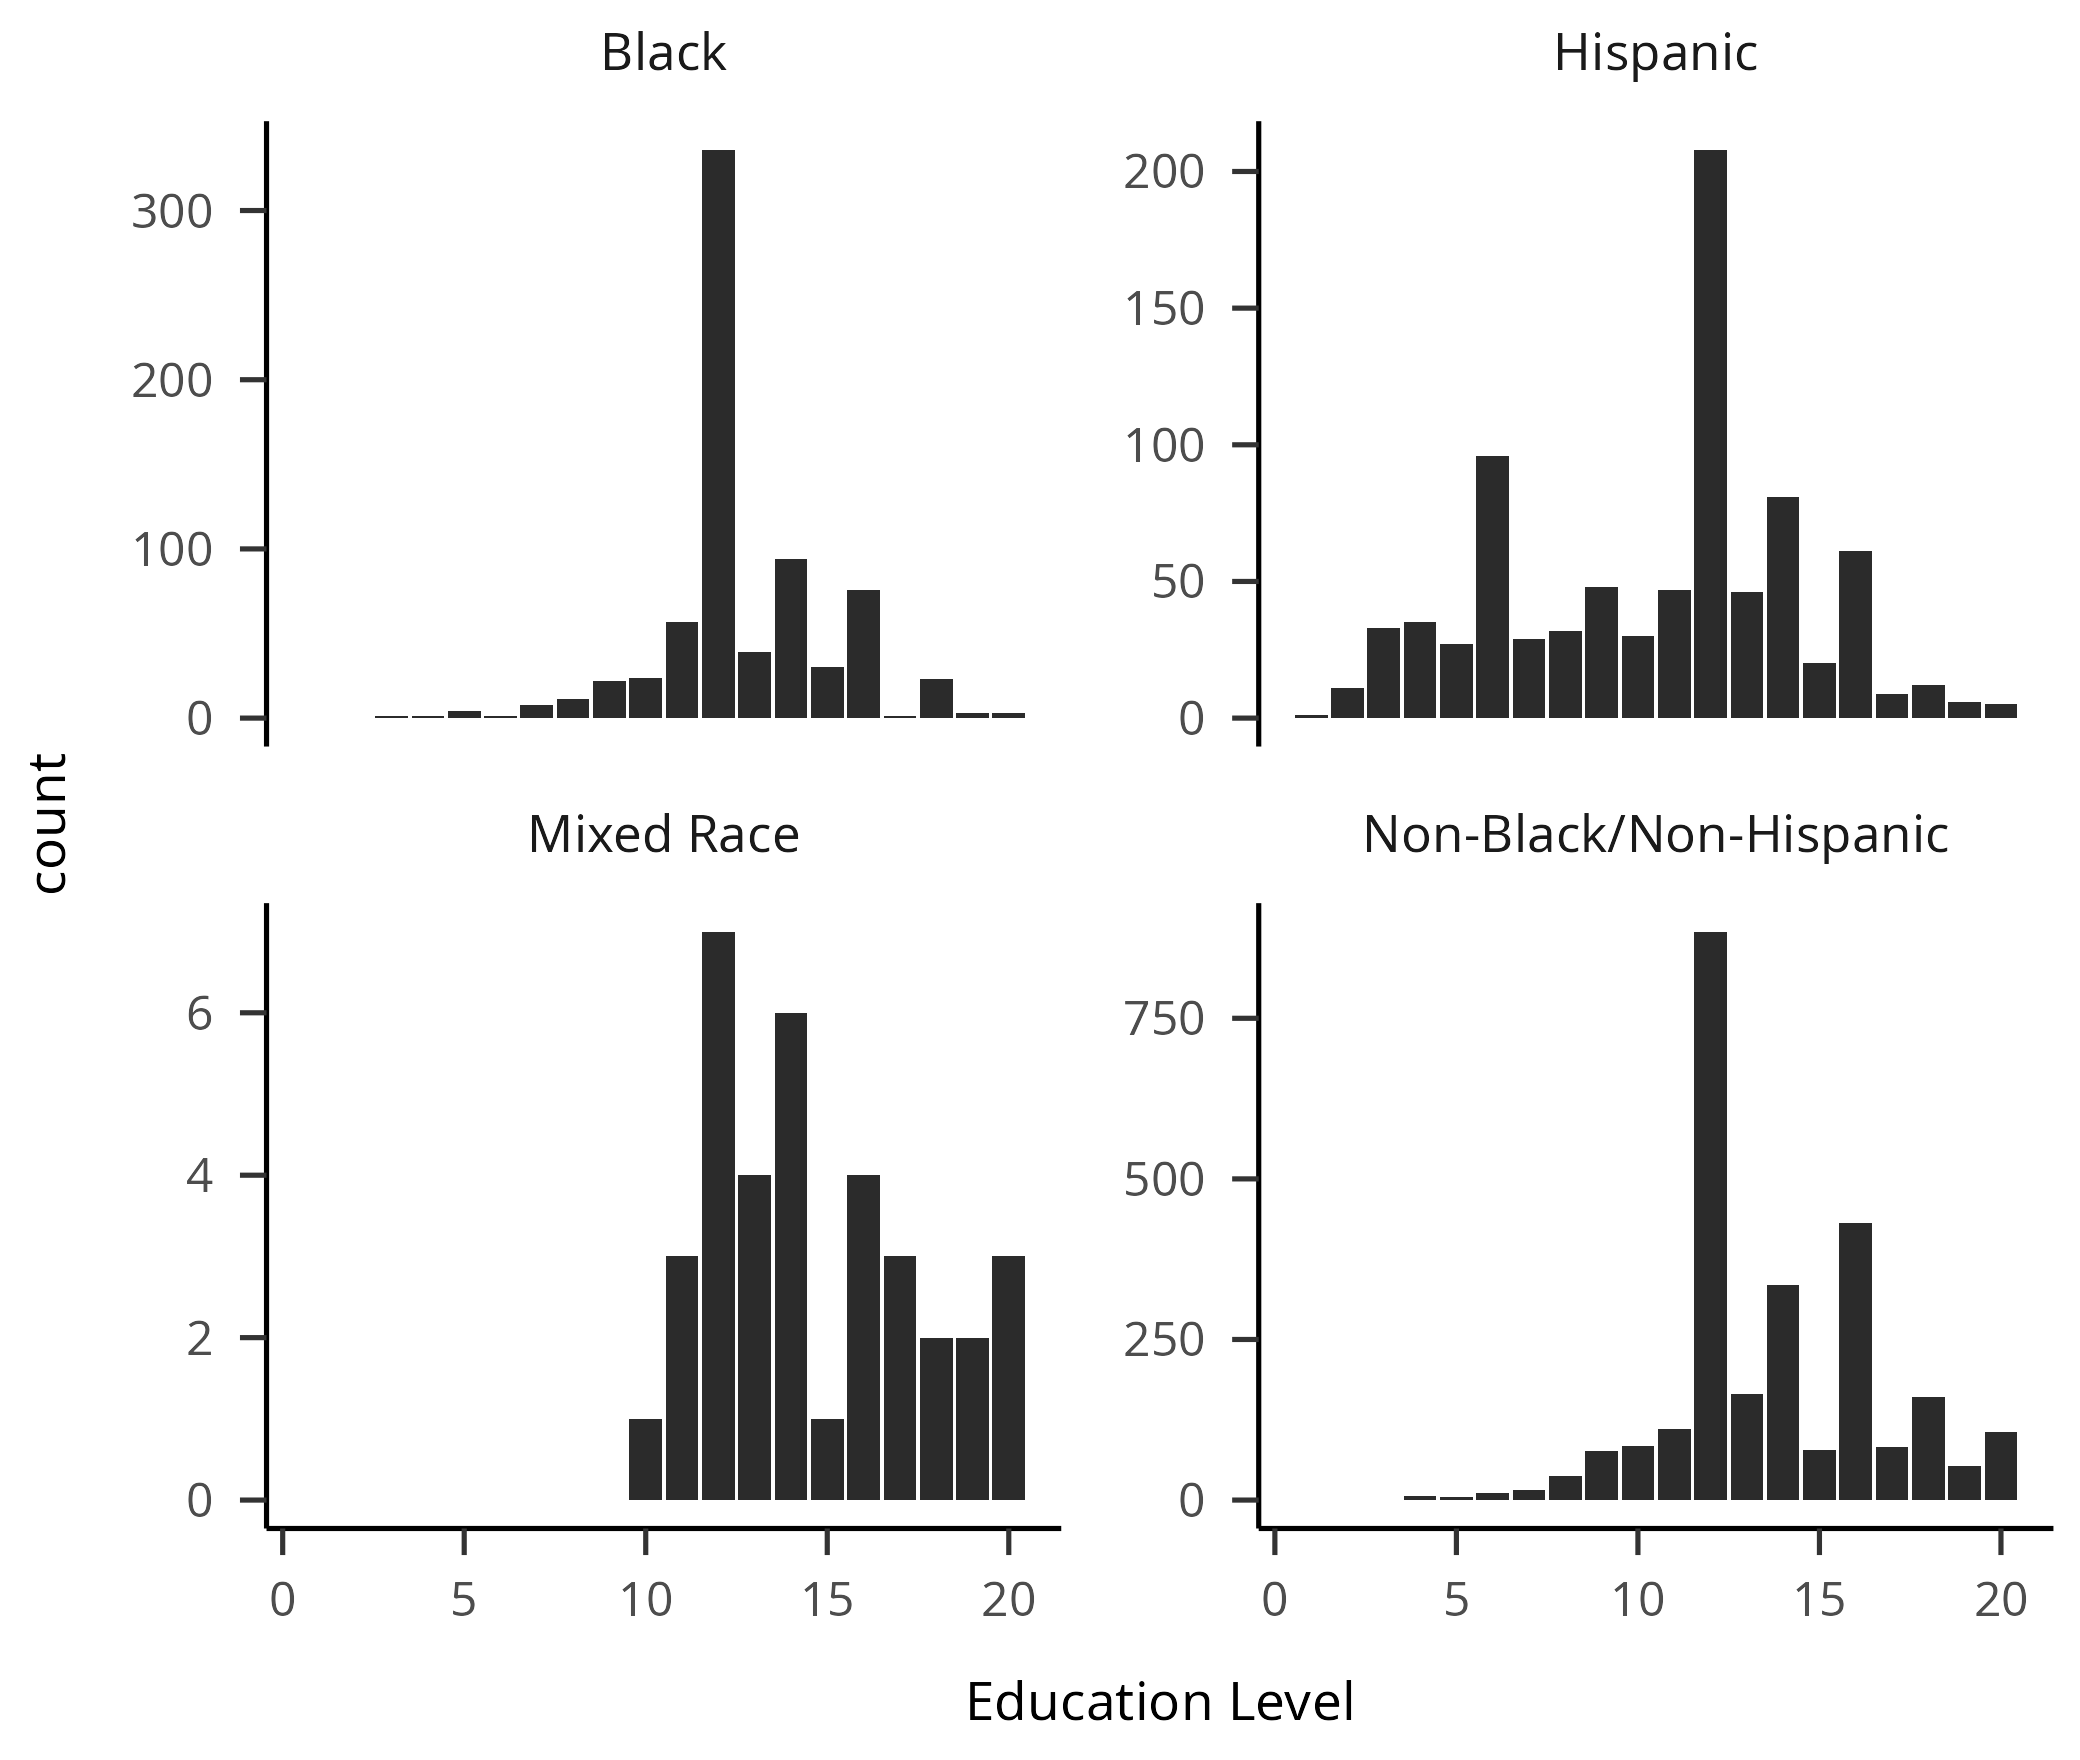
\includegraphics[width=\textwidth]{histogram3}
\end{figure*}

\begin{figure*}
  \caption{Upset plot of Missing Parental Education Values.}
  \label{Hist:Up}
  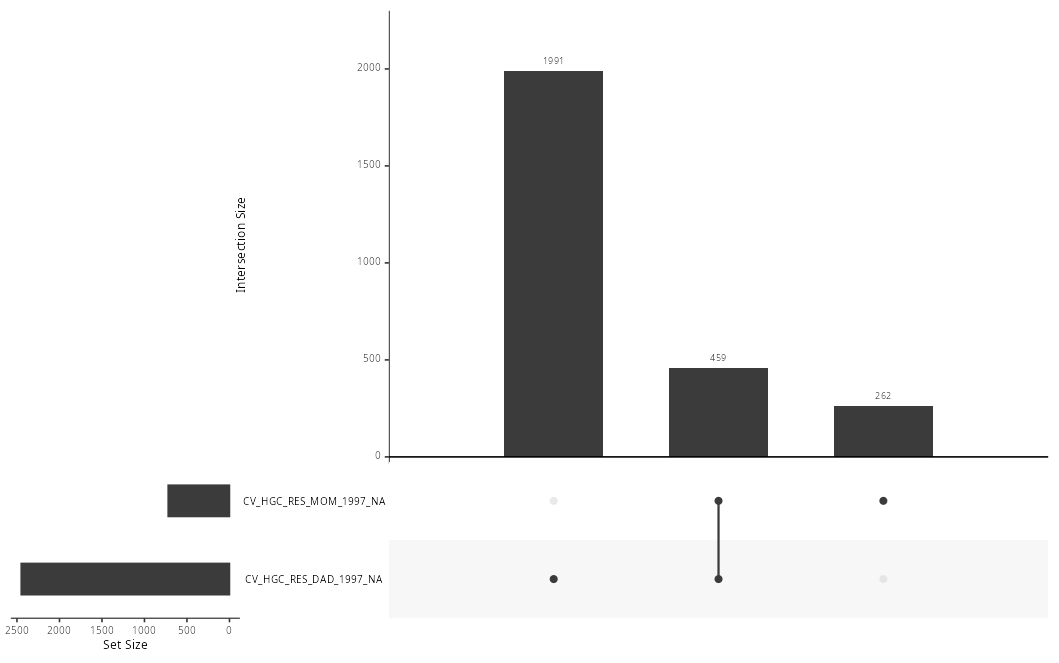
\includegraphics[width=\textwidth]{upset}
\end{figure*}

\begin{figure*}
  \caption{Imputation Vs Observed Value Density.}
  \label{Dens:Imp}
  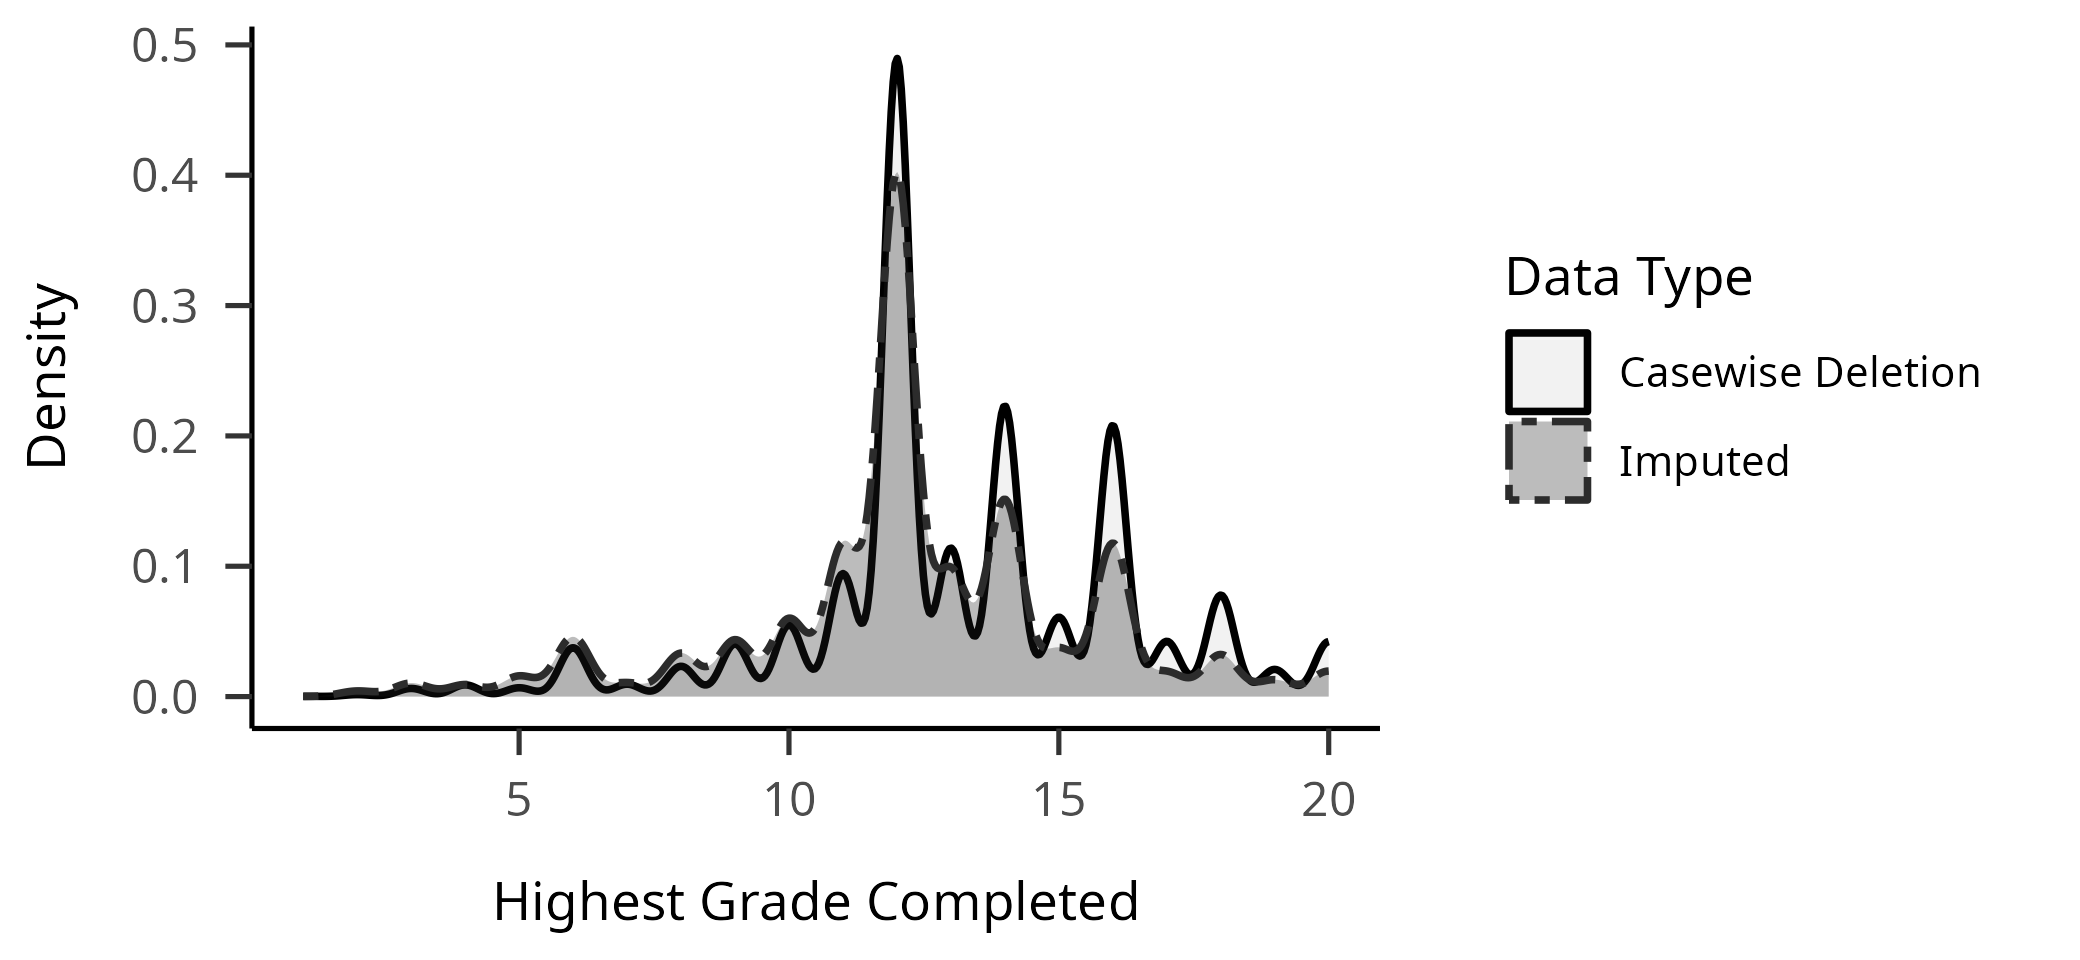
\includegraphics[width=\textwidth]{densityplot}
\end{figure*}

\section{Missing Mechanism Analyses}



\end{document}

%% 
%% Copyright (C) 2019 by Daniel A. Weiss <daniel.weiss.led at gmail.com>
%% 
%% This work may be distributed and/or modified under the
%% conditions of the LaTeX Project Public License (LPPL), either
%% version 1.3c of this license or (at your option) any later
%% version.  The latest version of this license is in the file:
%% 
%% http://www.latex-project.org/lppl.txt
%% 
%% Users may freely modify these files without permission, as long as the
%% copyright line and this statement are maintained intact.
%% 
%% This work is not endorsed by, affiliated with, or probably even known
%% by, the American Psychological Association.
%% 
%% This work is "maintained" (as per LPPL maintenance status) by
%% Daniel A. Weiss. 
%% 
%% This work consists of the file  apa7.dtx
%% and the derived files           apa7.ins,
%%                                 apa7.cls,
%%                                 apa7.pdf,
%%                                 README,
%%                                 APA7american.txt,
%%                                 APA7british.txt,
%%                                 APA7dutch.txt,
%%                                 APA7english.txt,
%%                                 APA7german.txt,
%%                                 APA7ngerman.txt,
%%                                 APA7greek.txt,
%%                                 APA7czech.txt,
%%                                 APA7turkish.txt,
%%                                 APA7endfloat.cfg,
%%                                 Figure1.pdf,
%%                                 shortsample.tex,
%%                                 longsample.tex, and
%%                                 bibliography.bib.
%% 
%%
%%
%% This is file `./samples/shortsample.tex',
%% generated with the docstrip utility.
%%
%% The original source files were:
%%
%% apa7.dtx  (with options: `shortsample')
%% ----------------------------------------------------------------------
%% 
%% apa7 - A LaTeX class for formatting documents in compliance with the
%% American Psychological Association's Publication Manual, 7th edition
%% 
%% Copyright (C) 2019 by Daniel A. Weiss <daniel.weiss.led at gmail.com>
%% 
%% This work may be distributed and/or modified under the
%% conditions of the LaTeX Project Public License (LPPL), either
%% version 1.3c of this license or (at your option) any later
%% version.  The latest version of this license is in the file:
%% 
%% http://www.latex-project.org/lppl.txt
%% 
%% Users may freely modify these files without permission, as long as the
%% copyright line and this statement are maintained intact.
%% 
%% This work is not endorsed by, affiliated with, or probably even known
%% by, the American Psychological Association.
%% 
%% ----------------------------------------------------------------------